\documentclass[a4paper,10pt]{article}
\usepackage{algorithm}
\usepackage{algpseudocode}
\usepackage{amsmath}
\usepackage{float}
\usepackage[margin=1in]{geometry}
\usepackage{graphicx}
\usepackage{hyperref}
\usepackage[utf8]{inputenc}

% amsmath clobbers this IEEE setting
\interdisplaylinepenalty=2500

\title{GPU and Hardware-Accelerated AES Encryption}
\author{Dominic DiPuma}

\begin{document}

\maketitle

\section{Introduction}

In recent years, encryption has become ubiquitous.  Smartphones and personal computers are often fully encrypted by default, and cryptography is being applied in new ways, such as for cryptocurrencies.  As a result, GPU, FPGA, and ASIC-accelerated cryptographic implementations are in focus.  On modern x86 and ARM processors, there are instructions to accelerate the advanced encryption standard (AES) algorithm.  This paper will describe the AES algorithm in enough detail to implement it, and study three custom implementations of the algorithm: a naive software implementation written in C; a C implementation using compiler intrinsics for the Intel AES instructions; and an Open Compute Library (OpenCL) implementation targeted at GPUs.  Each of the implementations will be profiled for their performance.  An implementation using the libgcrypt library will be studied as a reference.

\section{Technical Background}

AES is an encryption standard that was approved and published by the US government in the early 2000's.  Since it is a government-backed standard, it is thoroughly documented, and hardware implementations are even available in consumer electronics.  As such, it makes for an interesting case study in hardware acceleration.

From an implementation perspective, the AES algorithm is relatively simple.  At a high level, the algorithm has only a few elements:
\begin{itemize}
 \item A cryptographic key (either 128 bits, 192 bits, or 256 bits) is expanded several times (varies by key length), so that a different key is used at each ``round'' of encryption.  This expansion process is standardized, and is essentially a matrix multiplication followed by a byte substitution and then an XOR with a constant.
 \item The plaintext to be encrypted is broken up into 128-bit blocks, and each block is processed through several rounds.  Each round consists of a byte substitution, a shift operation, a matrix multiplication, and an XOR with that round's key.
\end{itemize}

How the 128-bit blocks are handled can vary depending on the specific cipher mode being used.  Popular modes for AES include electronic codebook (ECB), cipher block chaining (CBC), and counter (CTR)\cite{intel}.  ECB is the simplest of the group, and encrypts each block of plaintext on its own.  While ECB is the easiest mode to implement, the ciphertext produced can reveal repetition in the plaintext, so it is insecure.  CBC XORs the current block's plaintext with the previous block's ciphertext in order to remedy the security flaws of ECB.  Although this method is far more secure than ECB, it cannot be parallelized, since each block depends on its immediate predecessor.  This makes CBC a bad candidate for GPU acceleration.  The CTR mode encrypts a deterministically generated number, and then XORs the output with the plaintext.  The number can be produced by a simple counter or a pseudorandom sequence.  CTR can be parallelized, provided that the counter is parallel-safe.    This paper will implement the CTR mode, since it is parallelizable and is considered secure\cite{schneier}.

Additionally, the AES specification supports three different key lengths: 128-bit, 192-bit, and 256-bit.  Each key length uses a different number of encryption rounds per the specification (10, 12, and 14 rounds, respectively).  For this project, only the 128-bit version will be implemented.

\subsection{AES Encryption Algorithm}

Given a 128-bit block and the fully expanded key schedule (key expansion is described below), the AES algorithm consists of the following\cite{nist}:

\begin{algorithm}
\caption{AES-128 Encryption}
\begin{algorithmic}[1]
\Function{AesEncrypt128}{$input$, $output$, $key$, $counter$}

\State $state\gets$ $input$ + $counter$

\State $state\gets$ \Call{AddRoundKey}{$state$, $key$, $0$}

\State $round\gets 1$
\While{$round\leq 9$}
    \State $state\gets$ \Call{SubBytes}{$state$}
    \State $state\gets$ \Call{ShiftRows}{$state$}
    \State $state\gets$ \Call{MixColumns}{$state$}
    \State $state\gets$ \Call{AddRoundKey}{$state$, $key$, $round$}
    \State $round\gets round + 1$
\EndWhile

\State $state\gets$ \Call{SubBytes}{$state$}
\State $state\gets$ \Call{ShiftRows}{$state$}
\State $state\gets$ \Call{AddRoundKey}{$state$, $key$, $10$}

\State \Return $state$
\EndFunction
\end{algorithmic}
\end{algorithm}

The initial block can be viewed as a 4-by-4 matrix, where $A$ is a 16-byte array as in \eqref{block}.

\begin{equation}
 \begin{bmatrix}
  A[0] & A[4] & A[8] & A[12] \\
  A[1] & A[5] & A[9] & A[13] \\
  A[2] & A[6] & A[10] & A[14] \\
  A[3] & A[7] & A[11] & A[15] \\
 \end{bmatrix}
\label{block}
\end{equation}

Moreover, treating the current round key as a 16-byte array named $K$, the key is also a 4x4 matrix as in \eqref{key}.

\begin{equation}
 \begin{bmatrix}
  K[0] & K[4] & K[8] & K[12] \\
  K[1] & K[5] & K[9] & K[13] \\
  K[2] & K[6] & K[10] & K[14] \\
  K[3] & K[7] & K[11] & K[15] \\
 \end{bmatrix}
\label{key}
\end{equation}

\subsubsection{AddRoundKey}

\begin{equation}
 \begin{bmatrix}
  A[0] & A[4] & A[8] & A[12] \\
  A[1] & A[5] & A[9] & A[13] \\
  A[2] & A[6] & A[10] & A[14] \\
  A[3] & A[7] & A[11] & A[15] \\
 \end{bmatrix}
 =
 \begin{bmatrix}
  A[0] & A[4] & A[8] & A[12] \\
  A[1] & A[5] & A[9] & A[13] \\
  A[2] & A[6] & A[10] & A[14] \\
  A[3] & A[7] & A[11] & A[15] \\
 \end{bmatrix}
 \oplus
 \begin{bmatrix}
  K[0] & K[4] & K[8] & K[12] \\
  K[1] & K[5] & K[9] & K[13] \\
  K[2] & K[6] & K[10] & K[14] \\
  K[3] & K[7] & K[11] & K[15] \\
 \end{bmatrix}
\label{addroundkey}
\end{equation}

The AddRoundKey step is trivial.  The round key from the expanded key schedule is XORed with the block to form an updated block as shown in \eqref{addroundkey}.

\subsubsection{SubBytes}


\begin{equation}
 \begin{bmatrix}
  A[0] & A[4] & A[8] & A[12] \\
  A[1] & A[5] & A[9] & A[13] \\
  A[2] & A[6] & A[10] & A[14] \\
  A[3] & A[7] & A[11] & A[15] \\
 \end{bmatrix}
 =
 \begin{bmatrix}
  s[A[0]] & s[A[4]] & s[A[8]] & s[A[12]] \\
  s[A[1]] & s[A[5]] & s[A[9]] & s[A[13]] \\
  s[A[2]] & s[A[6]] & s[A[10]] & s[A[14]] \\
  s[A[3]] & s[A[7]] & s[A[11]] & s[A[15]] \\
 \end{bmatrix}
\label{subbytes}
\end{equation}

The SubBytes sub-function replaces every byte of the block with a unique byte from a standardized lookup table, denoted by the byte array $s$ in \eqref{subbytes}.  In the literature, this table is referred to as the ``s-box''.

\subsubsection{ShiftRows}

\begin{equation}
 \begin{bmatrix}
  A[0] & A[4] & A[8] & A[12] \\
  A[1] & A[5] & A[9] & A[13] \\
  A[2] & A[6] & A[10] & A[14] \\
  A[3] & A[7] & A[11] & A[15] \\
 \end{bmatrix}
 =
 \begin{bmatrix}
  A[0] & A[4] & A[8] & A[12] \\
  A[5] & A[9] & A[13] & A[1] \\
  A[10] & A[14] & A[2] & A[6] \\
  A[15] & A[3] & A[7] & A[11] \\
 \end{bmatrix}
\label{shiftrows}
\end{equation}

ShiftRows rotates each row of the block cyclically.  The "top" row is left alone, the next row is shifted by 1 byte, then 2 bytes, and the "bottom" row is shifted by 3 bytes as shown in \ref{shiftrows}.

\subsubsection{MixColumns}

\begin{equation}
 \begin{bmatrix}
  A[0] & A[4] & A[8] & A[12] \\
  A[1] & A[5] & A[9] & A[13] \\
  A[2] & A[6] & A[10] & A[14] \\
  A[3] & A[7] & A[11] & A[15] \\
 \end{bmatrix}
 =
 \begin{bmatrix}
  2 & 3 & 1 & 1 \\
  1 & 2 & 3 & 1 \\
  1 & 1 & 2 & 3 \\
  3 & 1 & 1 & 2
 \end{bmatrix}
  \begin{bmatrix}
  A[0] & A[4] & A[8] & A[12] \\
  A[1] & A[5] & A[9] & A[13] \\
  A[2] & A[6] & A[10] & A[14] \\
  A[3] & A[7] & A[11] & A[15] \\
 \end{bmatrix}
 \label{mixcolumns}
\end{equation}

MixColumns involves a matrix multiplication of the block with a standardized matrix as shown in \eqref{mixcolumns}.

This is not a ``typical'' matrix multiplication on 8-bit integers.  Instead, this is performed in in the Galois Field GF($2^8$) modulo 0x1b.  As far as computation goes, this means that multiplications are performed without carries, addition is replaced with XOR, and there is a modulus\cite{galois}.

Computing the new $A$ is shown in \eqref{mixcolumnex}.

\begin{align}
 \label{mixcolumnex}
 A[0] &= 2 \cdot A[0] \oplus 3 \cdot A[1] \oplus A[2] \oplus A[3] \\
 A[1] &= A[0] \oplus 2 \cdot A[1] \oplus 3 \cdot A[2] \oplus A[3] \\
 &\;\;\vdots \notag
\end{align}

Note that $\cdot$ is used to represent carryless multiplication with a modulus of 0x1b.  A similar expression can be found for each of the 16 bytes of $A$.

\subsubsection{Key Expansion}

Key expansion produces unique round keys for each round of encryption from the original 128-bit key.  These 11  round keys form the key schedule which is used throughout the entire encryption process (and therefore only needs to be calculated one time per key).

The first round key in the schedule is the original key.  From there, each round key is produced by manipulating the previous round key.  For the purposes of key expansion, the key is considered as an array of 4 32-bit words.

The first word in each round key is produced by taking the last word of the previous round key and then bit-manipulating it.  This word is rotated cyclically by one byte, and each of its bytes are substituted using the s-box from SubBytes.  Then, the word is XORed with a ``round constant''.  (Round constants are unique for each round of encryption.  The lower 3 bytes of each round constant are 0s, but the upper bytes are 0, then powers of 2 modulo 0x1b.  That is, the round constants are 0x00000000, 0x01000000, 0x02000000, ..., 0x1b000000, 0x36000000.)  Finally, this word is XORed with the first word of the previous round key,

The second, third, and fourth words of each round key are much simpler to calculate.  These are produced by XORing the previous word with the previous round key's Nth word.  For example, the second round key's second word is the second round key's first word XOR the first round key's second word; the second round key's third word is the second round key's second word XOR the first round key's third word; and so on.

\subsubsection{Counter}

For CTR mode, a counting sequence must be generated.  This can be any deterministic number sequence, but libgcrypt uses a big-endian 128-bit number which increments by 1 for each block.  This behavior will be replicated in order to have matching outputs between all implementations.

\subsubsection{AES Decryption}

Encryption and decryption are identical in CTR mode.  The plaintext can be obtained by XORing the encrypted counter sequence with the ciphertext.

\subsection{OpenCL}

OpenCL is a standard\cite{khronos} which is designed to enable parallel computing across GPUs, CPUs, and FPGAs.  Often, it is used to perform general purpose GPU computation.

An OpenCL program is made of a main executable and a ``kernel.''

The main executable is written in standard C or C++. This program's purpose is essentially to set up and launch the OpenCL kernel.  It makes API calls that query for OpenCL-compatible devices, creates an OpenCL context and a command queue on that device (or devices), compiles and loads a kernel onto the device(s), performs memory transfers inputs to the GPU, enqueues kernel commands, and transfers outputs from the GPU.  OpenCL will automatically determine how to distribute the enqueued kernel command across the available compute resources, and executes the kernel in parallel across many inputs.  

The kernel is a function written in OpenCL C and designed to execute in parallel.  In OpenCL C, a function can be made into a kernel by using the ``\_\_kernel'' qualifier before the function prototype.  Generally, the inputs and outputs to a kernel are arrays which are accessible to many kernel calls at once.  As a result, each kernel will generally work on a subset of array indices, which can be determined using the ``get\_global\_id'' function. For example, the 0th kernel ID may operate on array index 0, or on array indices 0 through 9; and the 1st kernel ID may operate on array index 1, or on array indices 10 through 19.  The decision about how to divide the work across kernels is left to the programmer.

Within kernels, OpenCL has more complex memory management than standard C does, and often requires variables to have explicitly declared address spaces.  There is ``\_\_global'' memory, which is accessible from the entire GPU, but is the most costly to access.  Alongside global memory is ``\_\_constant'' memory, which has the added restriction of being read-only.  ``\_\_local'' variables can be accessed from anything on the same execution unit, and this form of memory is faster and less abundant than global memory. The fastest but most sparse is ``\_\_private'' memory, which can only be accessed within a single function call.  ``\_\_private'' is the default for variables which are not explicitly labeled.

\subsection{Intel AES-NI}

Intel's instruction set extensions for AES include 6 instructions\cite{intel}. They perform the following tasks:

\begin{itemize}
 \item A single round of encryption
 \item The final round of encryption
 \item A single round of decryption
 \item The final round of decryption
 \item A single round of key expansion
 \item Invert the mix columns step (used to convert the encryption key schedule to the decryption key schedule)
\end{itemize}

Using these instructions, encrypting one block only requires an XOR, several calls to the encryption round instruction, and a final encryption round call.  Similarly, decrypting a block requires an XOR, several calls to the decryption round instruction, and a final decryption round instruction call.

Although requiring multiple calls to the round encryption functions sounds sub-optimal, it is important to note that each AES key length uses a different number of encryption rounds.  Not only would a one-instruction encryption command be difficult to implement in hardware, but it would make the instruction set more complicated.  Additionally, the instruction-per-round approach makes this instruction set flexible enough that it could be used on similar cryptographic algorithms.

Key expansion is a slightly more complicated operation.  The key expansion instruction that Intel provides only does part of the work.  Some byte-shifting and shuffling needs to be done separately, and the specific operations that are needed are described in Intel's whitepaper on AES-NI.  The inverse mix columns instruction allows for a key schedule to be converted into a decryption key schedule easily.

Since key expansion is only performed once per key, it is not necessary to optimize this operation as heavily as encryption and decryption rounds are optimized.  This is part of why manual byte-shifting and shuffling is considered acceptable.  The manual byte-manipulation steps are also useful because they enable the key expansion instruction to work with 128, 192, and 256-bit keys (as well as larger key lengths if AES grows in the future).

\subsection{libgcrypt}

Libgcrypt is the cryptography library developed for and used by GnuPG, which is a collection of free and open-source cryptography software.  The library includes multiple encryption algorithms, block modes, and key lengths.  As such, it is a good reference implementation of AES to benchmark the AES ciphers developed here ``from scratch.''

\section{Setup and Implementation}
 
\subsection{System Setup}

This was developed and tested on two systems:
\begin{itemize}
\item{A ThinkPad T450s laptop with an Intel Core i5 (Broadwell) 5200U dual core CPU.  This CPU includes an integrated Intel HD 5000 GPU and supports AES-NI instruction set extensions, as well as SSE 4.2 and AVX 2 vector instruction set extensions.  Hyperthreading is enabled to allow 4 simultaneous processor threads, and 128MB of RAM is dedicated to the integrated GPU in BIOS.  In terms of system software, the system is running Arch Linux which is up to date as of November 2020.  This includes Linux kernel 5.9.9, GNU Compiler Collection 10.2.0, glibc 2.32, and libgcrypt 1.9.2.}

\item{An Amazon Web Services (AWS) Elastic Compute Cloud (EC2) instance.  Specifically, this instance was a g4dn.xlarge instance with 4 virtual Intel Cascade Lake CPUs, 16GB of RAM, and an NVIDIA Tesla T4 GPU.  The CPUs include AES-NI instructions, as well as all Intel vector instructions up to and including AVX-512.  The GPU has 16GB of memory and 2,560 CUDA cores.  An Amazon Linux 2 machine image with NVIDIA's Tesla drivers pre-installed was used.  This OS includes Linux kernel 4.14.214, GCC 7.3.1, glibc 2.26, and libgcrypt 1.5.3.}
\end{itemize}

The un-accelerated implementation should compile and run on any modern system with a C compiler and support for POSIX threads (pthreads).  The CPU-accelerated implementation requires Intel compiler intrinsics and hardware support for the AES-NI extension set, which is available on many modern Intel and AMD CPUs.  The GPU-accelerated implementation requires OpenCL 2.2 support in software and hardware.  Lastly, the libgcrypt implementation requires development headers and the libgcrypt library.  However, only the configurations discussed above have been tested.

\subsection{Implementation}

\subsubsection{Software-Only Implementation}

The software-only implementation is largely a translation of the specification's pseudocode into C.  Each major step in the AES algorithm is written as its own function, with an AesCipher128 function to encrypt an entire block.  Some meaningful optimizations are included in this implementation.

The Galois field multiplication is replaced by two 256-byte lookup tables (one for multiplication by 2 and another for multiplication by 3). This replaces one of the most computationally complex operations in the algorithm with a simple lookup.

Additionally, the ShiftRows step is performed using the ``shuffle'' GCC builtin.  This is faster than the naive approach of using temporary variables and then re-assigning bytes in the block as it takes advantage of an x86 shuffle SIMD instruction.  SIMD instructions are also used in AddRoundKey, which performs its XOR operation on the entire block using one 128-bit variable.

After disassembling an earlier iteration of the compiled code, it was found that most loops in the AES encryption function were not unrolled (even when using GCC's ``-funroll-all-loops'' option).  Loops were manually unrolled to achieve better performance.

Since the CPU implementation handles the blocks keys in a number of different ways (as a single 128-bit integer, as an array of bytes, and as a GCC vector type), these types are defined C unions. MixColumns can access the individual bytes of each block, ShiftRows can access the block as a vector, and the block behaves as a 128-bit integer in AddRoundKey.

\subsubsection{OpenCL Implementation}

The OpenCL version of the algorithm was derived from the software-only version.  The implementation of AES is almost identical, with a few notable exceptions.

The OpenCL code is essentially the CPU header file, with AesCipher128 implemented as a kernel, and its inputs declared as \_\_global.  Additionally, any instances of the C ``const'' qualifier are replaced by OpenCL's equivalent ``\_\_constant'' flag.  There are some minor variable type changes to support OpenCL's types, as OpenCL has vector types in the standard but excludes types such as ``uint8\_t'' in favor of types such as ``uchar''.  However, the optimizations described for the CPU implementation still apply to the OpenCL version.

One additional optimization made to the OpenCL code is in the main executable.  Instead of compiling the OpenCL immediately before executing it, the compilation is done in a separate executable, and the binary is saved.  The AES encryption program loads this binary from the hard disk to reduce overhead.

\subsubsection{AES-NI Accelerated Implementation}

The instructions greatly simplify the code needed to implement AES.  Aside from using the built-ins and implementing key expansion as described by Intel, the only optimization is manual loop unrolling.

\section{Results}

\begin{figure}[H]
 \begin{center}
  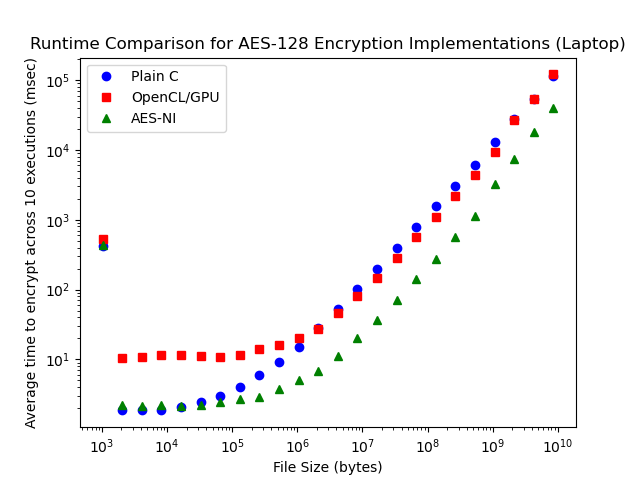
\includegraphics[width=\textwidth]{results_laptop.png}
  \label{plot_laptop}
  \caption{Runtime growth for all AES implementations on a laptop}
 \end{center}
\end{figure}

\begin{figure}[H]
 \begin{center}
  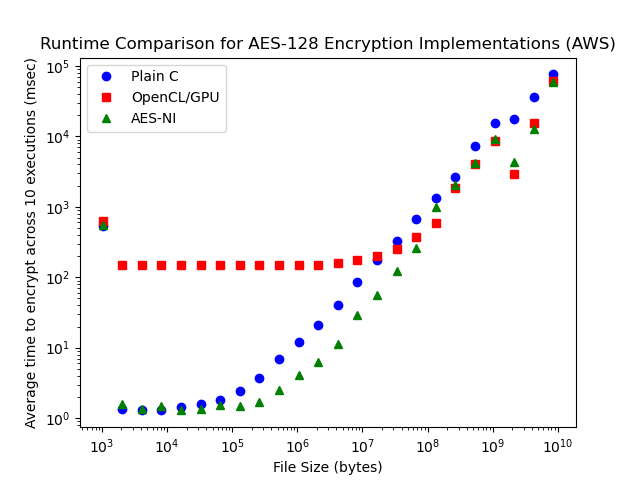
\includegraphics[width=\textwidth]{results_aws.png}
  \label{plot_aws}
  \caption{Runtime growth for all AES implementations on a laptop}
 \end{center}
\end{figure}

After executing all of the implementations several times on a range of file sizes, the average runtime for each implementation/size combination was plotted for both configurations.  Note that software-only and hardware-accelerated implementations were run using 4 simultaneous CPU threads.

\subsection{Analysis for Both Configurations}
In general, all implementations have linear runtime growth.  The algorithm for encrypting a single block is not influenced at all by the number of blocks, the data in the blocks, or the key.  Therefore, the algorithm's execution time should grow linearly with the number of blocks.

At small file sizes, the execution time does not change significantly as the file size increases.  This is because there are overhead costs to running these benchmarks.  All of these programs open/mmap two files (and later munmap/close them) and they derive the AES key schedule at runtime.  The pure C, AES-NI accelerated C, and libgcrypt implementations spawn pthreads, and the OpenCL program makes calls to gain access to the GPU and loads the AES algorithm onto it.  These operations should take the same amount of time to execute regardless of the file size, and with short execution times, the constant overhead dominates the expected linear runtime growth.

The runtime decrease from 1KB to 2KB is unexpected, and occurred consistently across executions and implementations.  This may be a quirk of handling 1KB files on the systems being studied.

In both configurations, the libgcrypt implementation performs nearly identically to the custom AES-NI program.  This makes sense, since the underlying library is optimized and uses the AES-NI instructions to perform encryption.

\subsection{Observations for the Laptop Configuration}

With the laptop's hardware/software setup, AES-NI is clearly the best performing program beginning at the 16KB  file size.  The GPU code has substantial overhead which limits its usefulness for small files, but it slightly outperforms the software-only program for sizes ranging from 2MB through 2GB. For the 4GB and 8GB file sizes, and the GPU-accelerated code is slightly slower than the software-only version.  This is likely due to the limited GPU memory on this device.

\subsection{Observations for the AWS Server Configuration}

Using the AWS server, the AES-NI accelerated implementation is the fastest for files below 128MB.  Beyond that point, the OpenCL version of the program is performance-competitive with the AES-NI application.  The pure software implementation is still generally the slowest (with the exception of small file sizes, where OpenCL's overhead dominates runtime).  However, the software-only version performs much more similarly to the AES-NI algorithm on the AWS server than it does on the laptop.  This is likely due to the availability of 512-bit vector instructions on the AWS machine's CPU, as well as other instruction optimizations made between Broadwell and Cascade Lake.

There is a strange dropoff in runtime between the 1GB and 2GB file sizes.  This occurred for all implementations, and may be a consequence of filesystem or network configuration on Amazon's servers.

% TODO - update

\section{Code Description}

Full source code is available on GitHub at \url{https://github.com/DDiPuma/Accelerated-AES-Benchmark}.

\subsection{Test Driver Software}

The outputs of each ``hand-written'' implementation were compared with the output of the libgcrypt library to prove that they produced identical output.

\subsection{Benchmark Software}

Benchmark executables were developed to run each AES implementation.  These programs use a hard-coded key and counter to eliminate the need to provide one as an input.  Memory-mapped input (i.e. plaintext) and output (i.e. ciphertext) files are used.  By using mmap() instead of read() and write(), the number of system calls is reduced substantially, which improves performance.

The software-only C, AES-NI accelerated, and libgcrypt-based C programs use POSIX threads (i.e. pthreads) to achieve parallelism.  Each thread runs a for-loop that encrypts one block per iteration.  Instead of using mutexes or any other synchronization method, the input and output files are broken up along cache line boundaries.  Since each cache line is accessed from only one thread, there are no data hazards, and synchronization is completely unnecessary.  Another benefit of this approach is that each thread is assigned a continuous span of memory, which improves data locality and therefore should improve the cache performance of the benchmark program.

The OpenCL version of the code performs some boilerplate OpenCL setup, including querying the system for devices and creating a context.  Afterwards, it loads a pre-compiled program onto the GPU, sets it up as a kernel, copies data from the input file to the GPU.  The encryption is placed on the GPU's queue, and once it completes execution, the outputs are copied back to the CPU to be stored.  OpenCL does not require any special considerations to be made to prevent data hazards.


\subsection{Scripts to Reproduce Output}

The source code includes several scripts to set up the system to run benchmarks.  After cloning and cd'ing into the the git repository, executing ``scripts/build.sh'' will compile all of the programs into the ``bin'' directory. Running ``scripts/make\_inputs.sh'' will generate pseudorandom files ranging from 1 kilobyte to 8 gigabytes in the ``input'' directory and will create an ``output'' directory.

Additionally, the scripts which execute the benchmarks and generate the results plot are provided.  Executing ``scripts/run\_bench.py'' will execute all four benchmarks 10 times per input file.  It then outputs the average runtime for each implementation and file size combination.  Copying this output into the ``scripts/plot.py'' program and then executing it provides the final plot.

\subsection{Other Utility Programs}

There is another program in ``bin'', which calculates complete lookup tables for each byte multiplied by 0x2 and 0x3 in GF($2^8$) modulo 0x1b.  This output is used in the source code as an optimization for the software-only and GPU implementations.

\subsection{Future Work}

There are several aspects of this project which can be studied further.

The possibility of encrypting multiple blocks in one function call should be explored, instead of encrypting each block independently in a for-loop. This may optimize performance by removing some branch instructions and even allowing the compiler to identify optimizations using SIMD instructions.  However, this approach may have limited benefits, as the highly-optimized libgcrypt implementation performs similarly to the custom AES-NI implementation.

The OpenCL/GPU code might have opportunities for further optimization.  Experimenting with kernel size and memory synchronization options may allow for better performance than relying on the defaults.

Additionally, the implementations presented here may be vulnerable to side-channel attacks.  Testing and improving the security of the programs would make them more practical for day-to-day use.

\bibliographystyle{ieeetr}
\bibliography{aes}


\end{document}
